\pgfplotsset{
    matrix plot/.style={
        axis on top,
        clip marker paths=true,
        scale only axis,
        height=\matrixrows/\matrixcols*\pgfkeysvalueof{/pgfplots/width},
        enlarge x limits={rel=0.5/\matrixcols},
            enlarge y limits={rel=0.5/\matrixrows},
            scatter/use mapped color={draw=mapped color, fill=mapped color},
            scatter,
        point meta=explicit,
        mark=square*,
        cycle list={
            mark size=0.5*\pgfkeysvalueof{/pgfplots/width}/\matrixcols
        }
    },
    matrix rows/.store in=\matrixrows,
    matrix rows=10,
    matrix cols/.store in=\matrixcols,
    matrix cols=10
}
  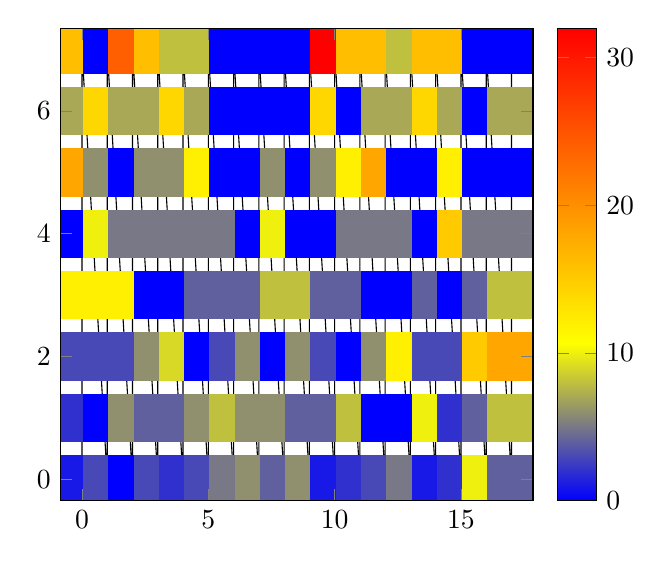
\begin{tikzpicture}
    \begin{axis}[
            width=60mm, 
            matrix plot,
            colormap/hot,
            colorbar
        ]
      \addplot table [meta=funceval] {
ppm popsize funceval
0 0 1
0 1 2
0 2 3
0 3 12
0 4 0
0 5 18
0 6 7
0 7 16
1 0 3
1 1 0
1 2 3
1 3 12
1 4 10
1 5 6
1 6 14
1 7 0
2 0 0
2 1 6
2 2 3
2 3 12
2 4 5
2 5 0
2 6 7
2 7 24
3 0 3
3 1 4
3 2 6
3 3 0
3 4 5
3 5 6
3 6 7
3 7 16
4 0 2
4 1 4
4 2 9
4 3 0
4 4 5
4 5 6
4 6 14
4 7 8
5 0 3
5 1 6
5 2 0
5 3 4
5 4 5
5 5 12
5 6 7
5 7 8
6 0 5
6 1 8
6 2 3
6 3 4
6 4 5
6 5 0
6 6 0
6 7 0
7 0 6
7 1 6
7 2 6
7 3 4
7 4 0
7 5 0
7 6 0
7 7 0
8 0 4
8 1 6
8 2 0
8 3 8
8 4 10
8 5 6
8 6 0
8 7 0
9 0 6
9 1 4
9 2 6
9 3 8
9 4 0
9 5 0
9 6 0
9 7 0
10 0 1
10 1 4
10 2 3
10 3 4
10 4 0
10 5 6
10 6 14
10 7 32
11 0 2
11 1 8
11 2 0
11 3 4
11 4 5
11 5 12
11 6 0
11 7 16
12 0 3
12 1 0
12 2 6
12 3 0
12 4 5
12 5 18
12 6 7
12 7 16
13 0 5
13 1 0
13 2 12
13 3 0
13 4 5
13 5 0
13 6 7
13 7 8
14 0 1
14 1 10
14 2 3
14 3 4
14 4 0
14 5 0
14 6 14
14 7 16
15 0 2
15 1 2
15 2 3
15 3 0
15 4 15
15 5 12
15 6 7
15 7 16
16 0 10
16 1 4
16 2 15
16 3 4
16 4 5
16 5 0
16 6 0
16 7 0
17 0 4
17 1 8
17 2 18
17 3 8
17 4 5
17 5 0
17 6 7
17 7 0  
      };
    \end{axis}    
  \end{tikzpicture}